\section{Experiments}\label{sec:experiments}
We first account for the training lineage of the evaluated CDPR controller and the skills measured along it. We then report skill retention during base-policy learning, the auxiliary LIBERO-Spatial feedback study, and complete-task CDPR adaptation. A WX200 evaluation is ongoing.

The CDPR simulation uses MuJoCo Warp/MJ-Lab, four object categories (apple, orange, potato, and tomato), and plate or bowl destinations. Full-task stages use 8-action chunks with a 4-action executed prefix, groups of 8 rollouts per scene, a 128-decision horizon, and 512 parallel worlds per GPU on two A40 GPUs. The continuation S11 uses a fresh Adam optimizer, learning rate $10^{-5}$, one PPO epoch per update, and initial $\log\sigma=-1.2$; its last 20M actions took 95.3\,h. Rewards, milestones, and training-only assistance read simulator state. The evaluated policy observes only the two camera images, proprioception, and the instruction.


\subsection{Training Lineage and Data Origin}\label{sec:lineage}
Table~\ref{tab:lineage} traces the evaluated controller from the pretrained model. Approach, pickup, and placement were acquired by RL with dense rewards (S1--S3), and retention cycles consolidated them by self-imitation on the policy's own successes (S4). No consolidated policy completed the full task, so two supervised stages seeded composition. S5--S6 fitted a scripted simulator oracle's pick-and-place trajectories. The oracle sets only the executed actions; observations, priors, resets, and predicates are the trainer's own. S9 fitted chains of earlier learned skill policies whose execution was assisted by scripted yaw, gripper-hold, and descent controllers, with every chain relabelled to the final instruction. Milestone RL then trained the policy without assistance (S10--S11).

Thus no human demonstrations or interventions on the CDPR enter the lineage, but automatically generated demonstrations do. The full-task result is not evidence for adaptation from the learner's own RL trajectories alone. Across S10--S11, full-task training consumed about 116M selected environment actions. Earlier stages and the oracle and chain collection add more, and some of their budgets were not retained. The unadapted model, pretrained SmolVLA with a fresh residual, was not evaluated under the full-task protocol. The earliest strict full-task measurement is 2.6\% at the start of S10, after both seeding stages.
% Source: evidence/DATA_LINEAGE_AUDIT_20261029.md. Interactions are selected
% environment actions where reported; n.r. = not reported in local evidence.
\begin{table*}[!t]
\caption{Training lineage of the evaluated CDPR controller, from the pretrained model (top) to the reported endpoint (bottom). No stage used human demonstrations or interventions on the target robot.}
\label{tab:lineage}\centering\footnotesize
\setlength{\tabcolsep}{3pt}
\begin{tabular}{@{}P{3.1cm}P{1.1cm}P{3.6cm}P{4.3cm}P{3.2cm}r@{}}\toprule
Stage & Parent & Objective & Supervised action targets & Training-only assistance & Interactions\\\midrule
S0 SmolVLA + new residual & --- & Pretrained VLA; residual default init. & --- (SO100 pretraining only) & --- & ---\\
S1 Approach & S0 & RL, dense distance reward & --- & Distance curriculum & 5.0M\\
S2 Pickup & S1 & RL, dense & --- & Gripper aligned above object & n.r.\\
S3 Placement & S1/S2$^*$ & RL, dense & --- & Object already held & 15M\\
S4 Retention cycles 1--3 & S3 & Family RL alternated with $\mathcal L_{\rm SI}$ & Own successful rollouts & Held/aligned starts in bank & n.r.\\
S5 Composition seed & S4 & $\mathcal L_{\rm SI}$ (residual) & Own successes + \textbf{scripted-oracle} pick-and-place & Oracle drives the robot & SFT only\\
S6 Re-harvested seed & S5 & $\mathcal L_{\rm SI}$ (residual) & As S5, larger oracle slice & As S5 & SFT only\\
S7 Joint sparse RL & S6 & RL, one binary reward, four instructions & --- & Mixed held/desk starts & 2.0M\\
S8 Release-recovery RL & S7 & RL, binary & --- & Gripper aligned above object & 2.1M\\
S9 Three-stage seed & S8 & $\mathcal L_{\rm SI}$ (residual, then expert LoRA) & Earlier policies chained with \textbf{scripted controller assistance}, relabelled & Handoffs between policies & SFT only\\
S10 Milestone RL & S9 & Milestone RL, residual only & --- & None (empty start, final prompt) & 56.1M\\
S11 Continuation & S10 & Milestone RL, offset-conditioned likelihood & --- & None & 60.0M\\\bottomrule
\end{tabular}\\[2pt]
\raggedright\footnotesize Interactions are selected environment actions; n.r.: not reported in the retained records. $^*$Exact parent not reconstructed. Oracle and assisted-chain collection budgets are not included.
\end{table*}

% Source: CDPR_CONSOLIDATED_PROGRESS_REPORT.md, "Instruction success by phase and
% retention cycle" and ledger entries; stage labels follow tables/lineage.tex.
\begin{table*}[!t]
\caption{Skill success by stage, in percent, with successes/attempts where recorded. Rows use different protocols (column P) and must not be read as one learning curve. ---: not measured, not zero.}
\label{tab:skill_matrix}\centering\scriptsize
\setlength{\tabcolsep}{2.5pt}
\begin{tabular}{@{}llcccccc@{}}\toprule
Stage & P & Reach & Pickup & Plate, held & Bowl, held & Plate, full task & Bowl, full task\\\midrule
S1 approach reference & D & 63.0 (645/1024) & --- & --- & --- & --- & ---\\
S2 pickup reference & D & --- & 26.0 & --- & --- & --- & ---\\
S3 placement, 15M & D & --- & --- & 71.0 & 32.0 & --- & ---\\
S4 before cycle 1 & B & 8.0 & --- & 50.0 & 23.1 & --- & ---\\
S4 after cycle 1 & B & 31.1 & --- & 52.3 & 27.7 & --- & ---\\
S4 after cycle 2 & B & 43.2 & 17.4 & 34.6 & 17.0 & --- & ---\\
S4 after cycle 3 & B & 47.8 (734/1536) & 11.9 (183/1536) & 73.8 (632/856) & 53.5 (364/680) & 0.5 (10/2168)$^\dagger$ & 1.1 (22/1928)$^\dagger$\\
S5 composition seed & B & 48.0 (737/1536) & 14.9 (229/1536) & 71.5 (612/856) & 47.9 (326/680) & 9.3 (80/856)$^\dagger$ & 2.6 (18/680)$^\dagger$\\
S7 joint sparse RL & B & 42.0 (168/400) & 14.7 (225/1536) & --- & --- & 50.0 (228/456)$^\dagger$ & 21.6 (76/352)$^\dagger$\\\midrule
S10 start (after S9) & V & --- & --- & --- & --- & 1.4 (7/512) & 3.9 (20/512)\\
S10, best separate eval. & E & --- & --- & --- & --- & 37.4 (46/123) & 33.8 (45/133)\\
S11 endpoint & V & --- & --- & --- & --- & 76.8 (393/512) & 64.5 (330/512)\\\bottomrule
\end{tabular}\\[2pt]
\raggedright\footnotesize P: D, dedicated skill reference; B, bank-harvest evaluation at registered caps; V, in-run strict full-task validation panel; E, separate strict evaluation on 256 distinct scenes. Full-task entries below the rule use an empty-gripper start and the strict criterion. $^\dagger$Earlier composed protocol: object on the desk 0.06--0.10\,m from the receptacle, scored by the earlier composed predicate. This differs from the strict full task.
\end{table*}


Table~\ref{tab:skill_matrix} records skill success along the lineage. Every component skill was measured above zero before full-task RL, and the same policy later executed the complete task. The rows use different instructions, resets, and success predicates; they document development and retention, not a single learning curve. They also do not show that instruction balancing improved later composition, which would require a control trained without it.

\subsection{Base-Policy Skill Learning and Retention}\label{sec:skill_retention}
These measurements concern dense-reward training of simple CDPR skills and their consolidation into a base policy (S1--S4), before full-task composition. Each skill uses the instruction and reset protocol in Section~\ref{sec:skill_acquisition}; placement tests start with the object already held. Learning a new skill can degrade previously learned behavior, which full-task execution later needs.

In a forgetting evaluation, mean reaching success falls from 64.1\% for the reaching reference to 5.3\% after placement RL, over three evaluation rounds per condition. The recovery evaluation in Fig.~\ref{fig:retention} is a separate measurement: balanced self-imitation raises reaching success from 8.0\% to 31.1\%. Plate placement changes from 50.0\% to 52.3\%, and bowl placement from 23.05\% to 27.65\%. The bank combines earlier reaching successes with current placement successes, balancing the retained data by instruction.

\begin{figure}[!t]
\centering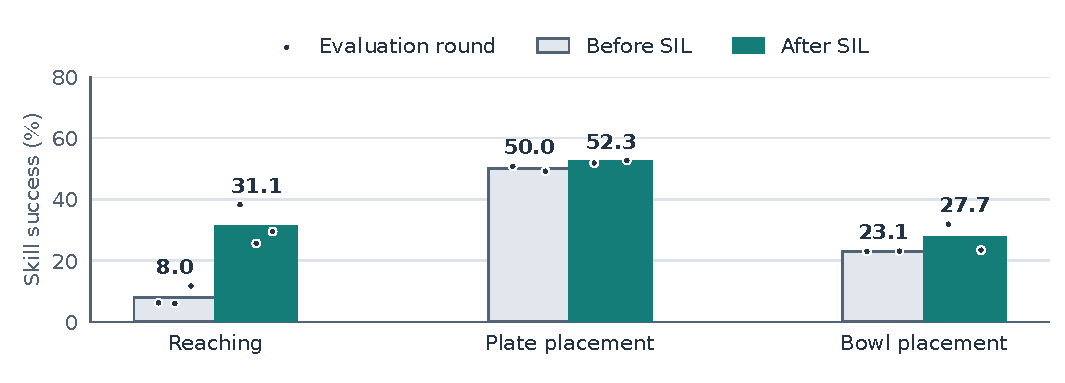
\includegraphics[width=\columnwidth]{figures/skill_retention.pdf}
\caption{Base-policy skill recovery before full-task composition. Bars show means and points show individual evaluation rounds: three for reaching and two for each placement skill, per condition. Reaching uses the instruction \emph{move to \textless object\textgreater}; placement starts with the object already held. Reaching partially recovers while both placement means increase.}
\label{fig:retention}
\end{figure}

Recovery is partial, with placement performance retained while reaching improves. These measurements cover approach and placement. They do not isolate the contribution of self-imitation to final full-task success, and no unbalanced-replay control was run.


\subsection{Auxiliary Study: Intermediate Feedback on LIBERO-Spatial}\label{sec:libero_results}
This study examines one question in isolation: whether intermediate feedback helps full-task RL. It uses a different backbone and does not run the adaptation schedule. It also does not test the milestone credit rule of Section~\ref{sec:composition}.

We fine-tune an OpenVLA-OFT policy with LoRA on complete instructions for the ten LIBERO-Spatial tasks~\cite{openvlaoft,libero}, using our own implementation of SimpleVLA-RL~\cite{simplevlarl}. The terminal-only row is our run under this study's budget, not a result from the SimpleVLA-RL publication. All runs start from one shared checkpoint with 61.0\% success; their final rates are measured after training. Each endpoint uses 300 validation rollouts from one training seed. The dense-plus-phase and terminal-only runs share terminal verifier coefficient 5 and 160 updates. The phase-only run differs in terminal coefficient (1), phase weight, and budget (110 updates), so we report it as a separate configuration rather than as a matched ablation. Dynamic sampling can make equal update counts consume different numbers of rollouts. Environment interactions and GPU-hours per run were not retained, so we compare runs only by updates.

From the shared 61.0\% initial policy, dense-plus-phase feedback reaches 65.3\% after 160 updates, against 61.7\% for terminal-only reward (Table~\ref{tab:libero}). With 300 rollouts, each endpoint's 95\% interval spans about $\pm$5.5 points, so the 3.6-point difference is not resolved by this single-seed comparison. Phase-only feedback reaches 62.3\% under its separate configuration.

These results motivate, but do not establish, the reward choice in the adaptation schedule. The schedule uses binary milestones during full-task learning because a completion predicate is simpler to specify than a continuous progress function for every phase of a new task (Section~\ref{sec:dense_method}). The LIBERO data do not show that binary milestones outperform dense-plus-phase feedback.
\begin{table}[!ht]
\caption{LIBERO-Spatial feedback study (our runs, one seed each). All runs start from a shared 61.0\% policy; endpoints use 300 validation rollouts. CI: Wilson 95\% interval.}
\label{tab:libero}\centering\small
\setlength{\tabcolsep}{4pt}
\begin{tabular}{@{}lrrrr@{}}\toprule
Configuration & Upd. & Final & CI & $\Delta$\\\midrule
Initial policy & 0 & 61.0 & n.r.$^c$ & ---\\
Terminal only$^a$ & 160 & 61.7 & 56.1--67.0 & +0.7\\
Dense + phase & 160 & 65.3 & 59.8--70.5 & +4.3\\
Phase-only$^b$ & 110 & 62.3 & 56.7--67.6 & +1.3\\
\bottomrule
\end{tabular}\\[2pt]
\raggedright\footnotesize$^a$Our implementation of SimpleVLA-RL~\cite{simplevlarl}. $^b$Terminal coefficient 1 instead of 5; not a matched ablation. $^c$Rollout count not recorded. $\Delta$: change from the initial policy, in points.
\end{table}



\subsection{SmolVLA: Complete-Task Adaptation}\label{sec:cdpr_results}
Strict success requires grasp, held lift, intentional release, and correct placement, without carry slip or wrong-placement events. Each attempt starts with an empty gripper and uses one full-task instruction, without teacher assistance. All attempts, including numerical failures, remain in the denominator.

The reported endpoint is evaluated on the development validation panel used during training: 1,024 attempts, 512 plate and 512 bowl, from a fixed set of 128 scenes that is reused at every reading. The endpoint was not chosen by peak score; it is the final checkpoint of the continuation, and the panel peak (71.09\%) is not used.
The adapted controller completes 723 of 1,024 development validation attempts (70.61\% strict success). A binomial 95\% interval is 67.7--73.3\%. Each of the 128 panel scenes contributes eight correlated attempts, so this interval is optimistic. Physical grasp occurs in 92.48\% of attempts and held lift in 88.28\%. Completion rates are 393/512 (76.76\%) for plates and 330/512 (64.45\%) for bowls. Carry slips (16.70\%) and wrong placements (14.16\%) remain the main failure modes.

The most recent evaluation off this panel used the checkpoint after 40M continuation actions. On 512 scenes outside the panel, each repeated four times, it completed 1,258 of 2,048 attempts (61.43\%), against 1,056/2,048 (51.56\%) for the 20M checkpoint on the same scenes. A frozen evaluation of the endpoint on untouched scenes remains to be done, so we treat 70.61\% as a development result.


\subsection{Additional Embodiment: WX200}\label{sec:wx200}
An ongoing experiment applies the schedule to the five-DoF WX200 serial manipulator. Its configured pipeline starts again from pretrained SmolVLA with a new residual, in simulation, rather than transferring the CDPR controller. It therefore tests the schedule on another mechanism, not controller transfer. No WX200 simulation or hardware result is reported in this draft. The final account will record failures, interventions, resets, and training-data sources, and will keep simulation and hardware results separate.
% The WX200 placeholder figure (figures/wx200_slots.pdf, or figures/wx200/panel.pdf
% when supplied) is withheld until real apparatus and rollout images exist.

\subsection{Context and Scope of the Evidence}
Table~\ref{tab:context} places the CDPR result next to related pick-and-place and adaptation results. It is contextual, not a benchmark. Robots, objects, resets, horizons, and success criteria differ across rows, and similar task names do not imply the same task distribution. SmolVLA's score gives half credit each for grasp and placement~\cite{smolvla}; the CDPR score counts only complete strict successes. No row supports a claim of superior performance or sample efficiency.

\begin{table}[!t]
\caption{Contextual results across different settings; not a controlled comparison.}
\label{tab:context}\centering\footnotesize
\setlength{\tabcolsep}{2.5pt}
\begin{tabular}{@{}P{1.75cm}P{2.45cm}P{1.45cm}P{1.35cm}r@{}}\toprule
Work & Robot, task & Human target demos & Metric & Result\\\midrule
SmolVLA~\cite{smolvla} & SO100 (real), cube pick-place & 50/task, multitask & Partial credit & 75\%\\
SimpleVLA-RL~\cite{simplevlarl} & LIBERO-Spatial (sim.) & 1/task & Binary & 98.2\%\\
RL boot.~\cite{nurtdinov2026rlboot} & CDPR (sim.), move to object & 0 & Strict binary & 9.75\%\\
Ours & CDPR (sim.), put into plate/bowl & 0$^a$ & Strict binary & 70.61\%$^b$\\\bottomrule
\end{tabular}\\[2pt]
\raggedright\footnotesize$^a$Automatically generated supervised data in the lineage (Table~\ref{tab:lineage}). $^b$Development panel; off-panel 61.43\% at 40M continuation actions.
\end{table}

The evidence supports a feasibility claim: a pretrained VLA with a newly initialized residual reached 70.61\% strict full-task success on a simulated CDPR, with no human demonstrations collected on that robot. It does not attribute that result to any single stage. Three controls are still missing. The first is direct full-task RL from the same pretrained initialization and residual architecture, with the same information, evaluation, and total interaction budget, including the schedule's acquisition, consolidation-data, and composition interactions and its oracle and assisted data. The second compares protected with unprotected milestone credit from the same consolidated checkpoint. The third compares instruction-balanced with ordinary successful replay under the same data and optimization budget.

The result comes from one training lineage, so no training-seed variation is measured. The development panel was inspected during training, and a frozen evaluation on untouched scenes, with per-episode outcomes, is pending. We also have not tested whether the controller selects objects and destinations from language within a fixed scene. The LIBERO study shares neither the backbone nor the full schedule with the CDPR pipeline. Avoiding human demonstrations does not remove the engineering of simulator, rewards, resets, success predicates, oracle, and assisted controllers, nor the RL compute.

